

%/******************************************************************************
% *filename:		mokuaisheji.tex
% *author:  		synckey
% *version: 		v1.0
% *datetime:		2011-06-24 08:42:26
% *description:		模块设计
% *****************************************************************************/
\section{模块设计}
\subsection{线程设计} 
\subsubsection{工作线程设计} 
\par{
在系统开始运行时创建MAXDNSTHREADS个工作线程,放入线程池中。主线程创建监听套接字,开启服
务。每个线程各自调用accept,采用互斥锁来保证在每一个时刻只有一个线程调用accept。
每个线程在accept后为客户端服务。}
\par{由于TCP内部为监听套接字维护两个队列:a.已完成队列,b.未
完成队列。所以在主线程睡眠期间,新的客户连接会使这两个队列充满(两个队列之和不超
过在listen时指定的backlog),而在这两个队列满了之后当一个客户的SYN到达时,TCP就
忽略该分节,也就是说,并不返回RST。这样做是因为:这种情况是暂时的,客户将重发SYN
,期望在不久就能在这些队列中找到可用空间\cite{unpv1}。 所以当这两个队列充满以后
,客户只是重发SYN ,而服务器不会接受客户端创建更多的连接。}
\begin{figure}[H]
\centering
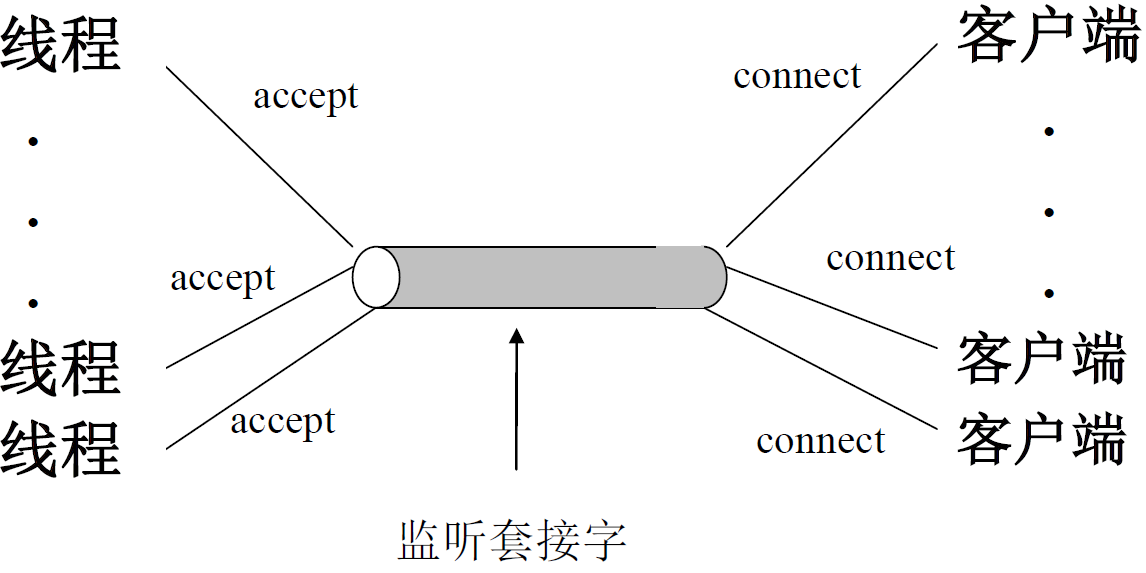
\includegraphics[keepaspectratio, scale=0.4]{pitures/xianchengmoxing.png}
\caption{工作线程模型} 
\end{figure}

线程池中的工作线程首先调用connect,接受一个客户端的连接,然后从报文的前4个字节中
获取报文的长度,从内存管理模块申请相应大小的内存,用于存放请求报文。
在收到请求后,逐次扫描每个域名。获得域名后,首先在本地的缓存中查找域名对应的IP,
如果有记录,就把IP地址填写到返回报文中,如果没有记录,则填入127.0.0.1,表明本地
没有缓存,把这个域名相应的序号和域名填入到下图所示的链表中,再进行DNS查询,结
果在第二个报文中返回。

\begin{figure}[H]
\centering
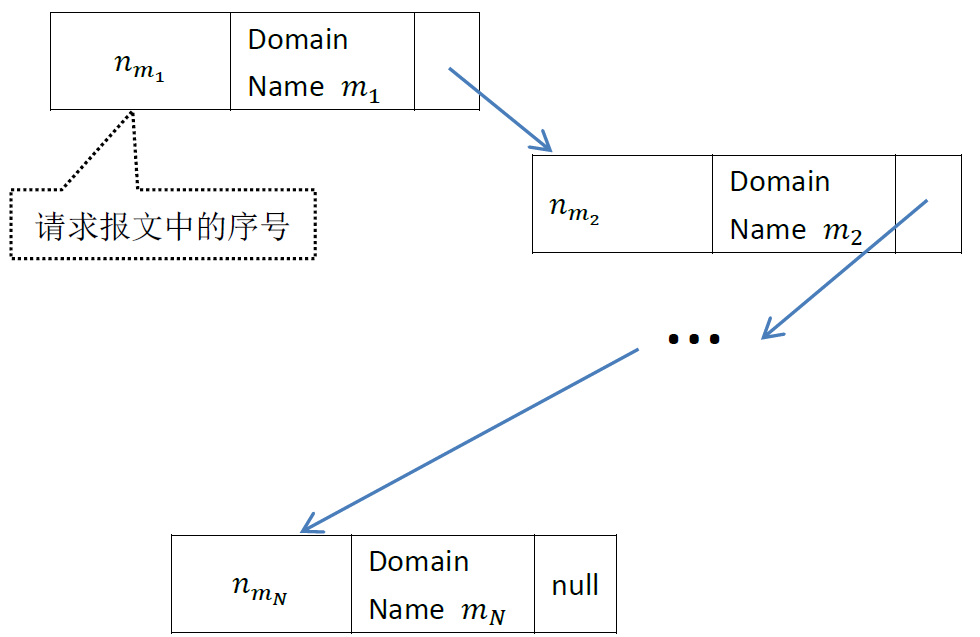
\includegraphics[keepaspectratio, scale=0.5]{pitures/response2_dns_list.png}
\caption{本地缓存未命中的域名构成的链表} 
\end{figure}

\par{工作线程在把请求报文遍历完毕后,就把第一次返回报文发送
给客户端,同时也把所有本地没有缓存的域名构造成了一个链表。如果链表为空,说明请求
的域名在本地都有缓存,任务完毕,关闭连接。否则,根据链表中的数目,申请用于构造第
二次返回报文的内存空间。对链表进行遍历,对链表中的每个域名和其对应的连接套接字将
其放入DNS线程的工作队列,由DNS查询线程执行查询操作。}

\begin{figure}[H]
\centering
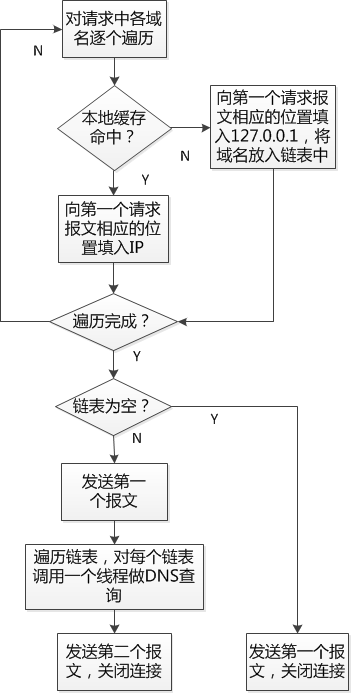
\includegraphics[keepaspectratio, scale=1]{pitures/xianchengliuchengtu.png}
\caption{线程工作流程图} 
\end{figure}

\subsubsection{DNS查询线程}
由于每个DNS请求只能请求单个域名,所以设计DNS查询线程来实现DNS的并发请求。DNS查询线程从
DNS工作队列中读取域名请求,然后对域名进行DNS查询,并将查询结果存入本地缓存。
对于同一个客户端的DNS查询,DNS查询线程检查它自己是不是该客户端的域名请求中最后一个完
成的,如果是最后一个完成的,就把查询结果发送给客户端并关闭TCP套接字。各个线程对
工作队列的并发访问通过互斥锁来保护。工作队列设计如下:
\begin{figure}[H]
\centering
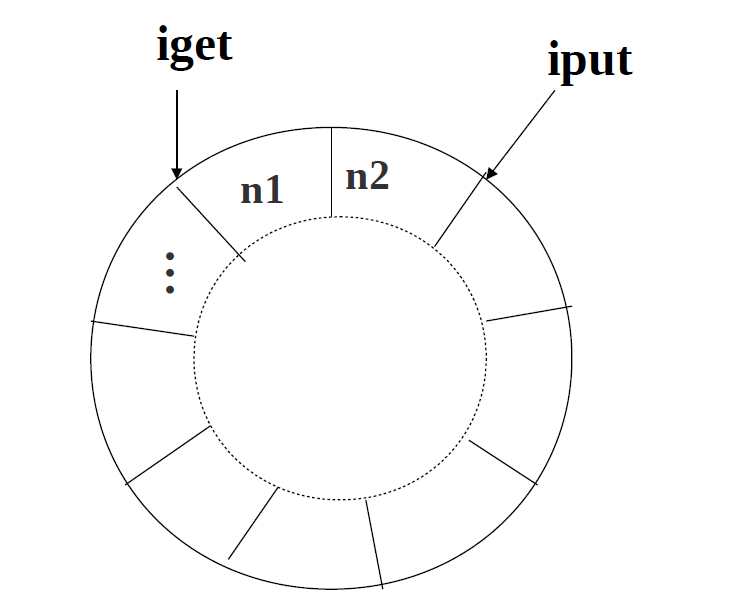
\includegraphics[keepaspectratio, scale = 0.4]{pitures/dnsxianchengduilie.png}
\caption{DNS线程工作队列} 
\end{figure}
其中iget表明下一次读取工作时的下标,iput表明由主线程在把工作时放入队列时的下一个
下标,对iput和iget的维护是在对工作队列加锁的情况下完成的。
\subsubsection{DNS服务器线程}
DNS服务器线程是一个单线程迭代服务器,运行在系统的主线程中。它迭代处理
客户端的请求,客户端根据它请求的域名个数来决定
使用UDP还是TCP来连接服务器。
\subsection{客户端测试模块}
客户端测试模块是提供给客户端的调用接口,它在内部与服务器交互。根据用户请求的域名
个数,它决定使用UDP还是TCP与服务器交互。
%%%%%%%%%%%%%%%%%%%%%%%%%%%%%%%%%%%%%%%%%%%%%%%%%
%                                               %
%filename	mm.tex				%
%author		wakemecn			%
%date		6/23/2011			%
%                                               %
%%%%%%%%%%%%%%%%%%%%%%%%%%%%%%%%%%%%%%%%%%%%%%%%%

%\documentclass{article}
%\usepackage{xeCJK}
%\setmainfont[BoldFont=SimHei]{SimSun%}
%\setmonofont{SimSun}
%\XeTeXlinebreaklocale"zh"
%\begin{document}
\subsection{内存管理模块}
		模块从系统预先申请256B,512B,1KB,2KB,$\ldots$,$2^n$KB等2幂次大小的块
		各若干。通过mem\_chunk结构维护特定大小的内存块大小的幂级,预分配的数目,
		已被使用的块链表和空闲的块链表。指针数组维护所有大小块的mem\_chuck结构
		指针。当申请使用M KB($2^m < M < 2^n$)空间时,若$2^n$KB大小块仍有空
		闲块,则将其分配,并将该块移动至已使用块链表中;若上述大小的块不存
		在空闲块或者不存在该大小的块,则模块动态申请若干数目该大小块的内存区域,
		分配内存。当释放某大小块时,若检测到释放的块位于模块动态申请的内存中
		时,则释放该内存。
\begin{figure}[H]
\centering
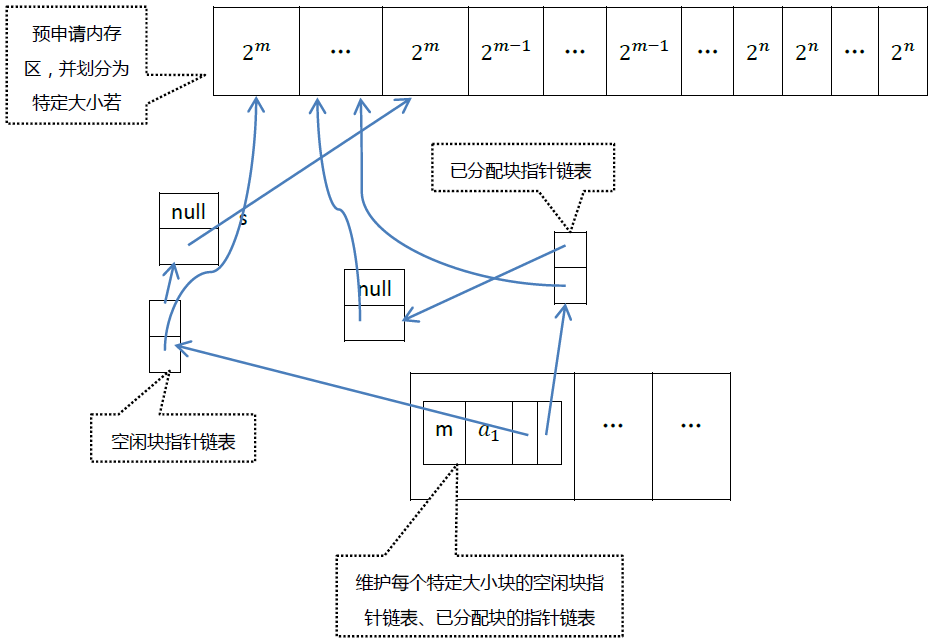
\includegraphics[keepaspectratio,scale=0.5]{pitures/mm.png}
\caption{内存管理示意图}
\end{figure}


%%%%%%%%%%%%%%%%	end of mm.tex    %%%%%%%%%%%%%%%


\subsection{缓存管理模块} 

缓存管理模块由DATrie和LIRS栈驱动。其中DATrie管理域名索引,域名对应的IP信息
保存在由LIRS管理的缓存中。当有域名查询请求时,从DATrie中查找到指定域名,返回保
存该域名的LIRS栈指针,从栈中取得IP信息。
\subsubsection{DATrie和LIRS的定义}
\noindent \textbf{DATrie:}双数组Trie(Double-Array Trie,DATrie)是trie树的一
个简单而有效的实现,虽然构造的代价很高,但是具有非常高效的查询效率。它由两整数数
组构成,一个是 base[],另一个是check[]。这两个数组间的关系如下:$$check[base[s] + c] = s$$
$$base[s]+ c = t$$


\begin{figure}[H]
\centering
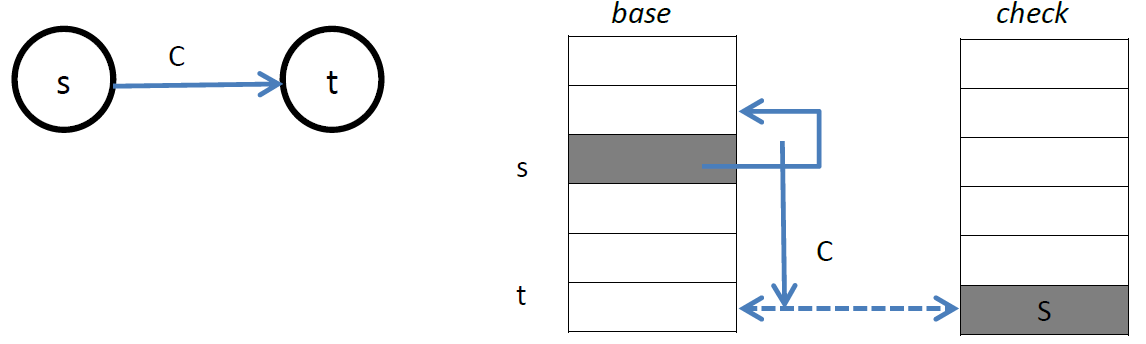
\includegraphics[keepaspectratio, scale=0.4]{pitures/aaa.png}
\caption{ DATrie 的状态转换示意} 
\end{figure}

\noindent \textbf{LIRS:}最短最近使用间隔算法(Low Inter-Reference Recency Set,LIRS): LIRS算法
	是一种基于LRU算法弱点而改进的算法,使用页面的最近使用间隔(Inter-Reference Recency,IRR)
	来决定要替换的页面。IRR用来表示一个页面的最近两次访问的间隔中的其他无重复页面的个数。
	LIRS还定义了最近访问时间R(Recency,R),用来表示一个页面的最近访问至当前访问之间
	的其它无重复页面的个数。


\begin{figure}[H]
\centering
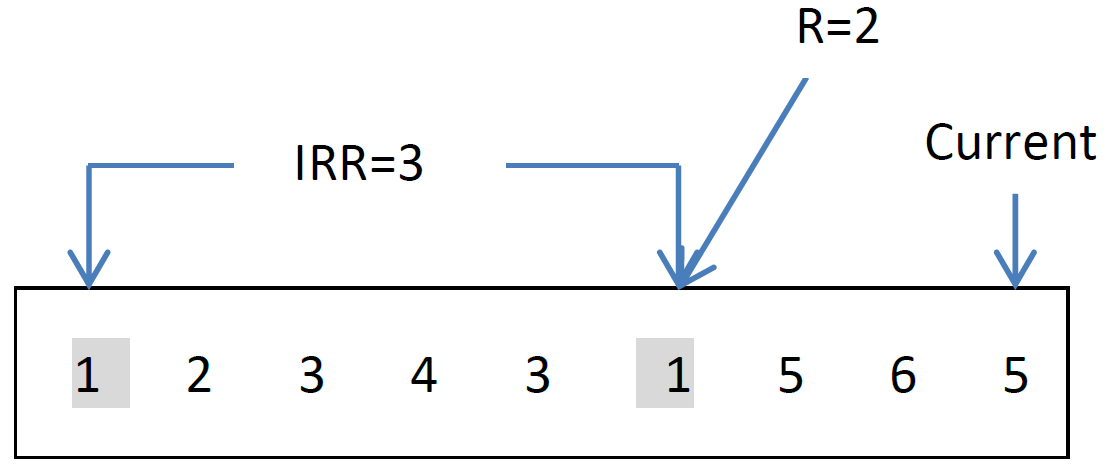
\includegraphics[keepaspectratio, scale=0.4]{pitures/irr.png}
\caption{LIRS算法的IRR和R的示意} 
\end{figure}

\paragraph{DATrie的实现\\[5pt]}
	对域名集合的索引是由两个DATrie驱动的。其中
	一个DATrie较大,是主字典树,存放所有已知域名集合,是系统在启动时从文件中
	读入信息构造的;另一个DATrie较小,是副字典树,实际应用中作为较大的
	DATrie的补充,是动态变化的。每当动态DATrie中记录达到一定数目时,就会离线
	补充到静态DATrie中,失效域名从静态DATrie中剔除。当有请求查询缓存时首先访问
	静态的DATrie,若没有命中则访问动态DATrie,当两者均未命中时选择向动态DATrie中插入记录。
	\par
	 {域名索引不仅是对缓存内容索引,可能缓存中不存在的域名也会被索引。 }
	 \par{由于DATrie内部实现的需要,要把域名对应的字符集转换成DATrie的内部编
	 码,对应关系如下表:}

\begin{table}[H]
\centering
\begin{tabular}{*{14}{|c}|}
\hline
\textbf{character}&a&b&c&d&e&f&g&h&i&j&k&l&m\\
\hline
\textbf{code}&1&2&3&4&5&6&7&8&9&10&11&12&13\\
\hline
\textbf{character}&n&o&p&q&r&s&t&u&v&w&x&y&z\\
\hline
\textbf{code}&14&15&16&17&18&19&20&21&22&23&24&25&26\\
\hline
\textbf{character}&-&.&0&1&2&3&4&5&6&7&8&9&\_\\
\hline
\textbf{code}&27&28&29&30&31&32&33&34&35&36&37&38&39\\
\hline
\end{tabular}
\caption{域名字符集和DATrie内部编码对应表}
\end{table}


\paragraph{LIRS算法的实现\\[5pt]}
LIRS算法的具体实现是由一个LIRS栈S和一个FIFO队列Q组成。LIRS栈S维护LIR块,同时也维护常驻或非常
驻状态的HIR块,FIFO队列Q维护所有常驻的HIR块。当需要替换时,替换HIR中的块,按先进
先出的顺序进行替换。
\begin{figure}[H]
\centering
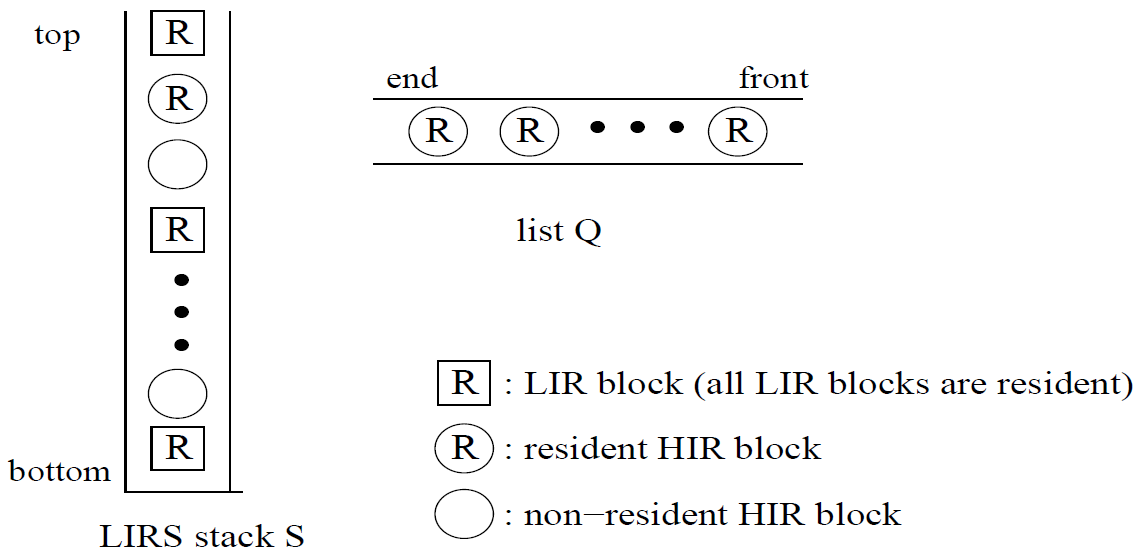
\includegraphics[keepaspectratio, scale=0.4]{pitures/lirsstack.png}
\caption{LIRS栈S和FIFO队列Q示意图} 
\end{figure}


%/************`*********************  END OF mokuaisheji.tex  *********************************/
